
% this file is called up by thesis.tex
% content in this file will be fed into the main document

% ----------------------- introduction file header -----------------------
\chapter{Motivation and theory framework}
\label{chapter:SM}
% ----------------------- paths to graphics ------------------------

% the code below specifies where the figures are stored
\graphicspath{Chapters/CH1/figures}
% -----------

The construction of the Standard Model is the result of a long series of experiments
and brilliant ideas in both theoretical and experimental fields.
Towards the end of the 1960s, knowledge of what we consider to be the constituent
elements of nature and the fundamental interactions among them, was organised
in the so-called Standard Model (SM).\\
More recently, a missing piece towards the completion of the SM, the Higgs boson,
was discovered by the ATLAS and CMS collaborations.\\
The ambition is to find a theoretical representation of all phenomena experimentally accessible.\\
Since particle physics is characterized by phenomena that are both relativistic
and quantistic, the description of the Standard Model relies on the
formalism of \textit{Quantum Field Theories} (QFT), synthesis of quantum mechanical
and relativistic theory. In these terms, the concept of field is associated
both to material particles and to forces. Particles are mere manifestations of
fields: they are identified with the quanta of the material fields and
force fields and the interaction among particles is determined by the exchange of virtual quanta of the field.\\
To search for extensions of the SM, it is possible to postulate a scale of the new physics high enough to manifest itself through deviations of known observables, usually at high energies.\\
In this chapter, a concise description of the SM will be presented, from the gauge
principle to the description of several theories of physics beyond the Standard Model which are crucial for the search of FCNC decay of the top quark.

% ----------------------------------------------------------------------
% ----------------------- introduction content -------------------------
% ----------------------------------------------------------------------


\section{The gauge principle in quantum field theory}

The mathematical framework of the SM is based on a quantum field theory description of the particles and their interactions.
The structure is a consequence of the invariance of physics under certain general symmetries:
these invariances are called \textit{gauge} because there is freedom in the choice of a certain number of parameters
that can precisely "calibrate" the model.
Each symmetry is therefore associated with a set of transformations that frame the "gauge group of the theory".
The theory is introduced starting from the Lagrangian formalism developed in the classical mechanism, extending this formalism to
classical field theory and finally to quantum field theory.
\vspace{\baselineskip}
 \\Lagrangian is defined as the difference between the kinetic energy and the potential energy of the system, as below:
\begin{equation}
\mathcal{L} (q,\dot{q}) =  \frac{m}{2}(\dot{q})^2-V(q)
\end{equation}
where $q$ is a set of generalized coordinates and $m$ is the mass of the particle.\\
The \textit{action} is defined as $ S = \int dt \mathcal{L} (q,\dot{q}) $.
\vspace{\baselineskip}
\\Using a variational approach it can be shown that for any possible variation of the path of the particle, $\partial(q)$,
the equation of motion of the system is  the one that minimizes the \textit{action}.
The results are the so called \textit{Euler-Lagrange} equations:
\begin{equation}
	\frac{\partial\mathcal{L}}{\partial q} -  \frac{d}{dt}\bigg(\frac{\partial\mathcal{L}}{\partial\dot{q}}\bigg)=0
\end{equation}
The next step is the extension of the classical mechanics formalism  to field theory. One possible way is to generalize 
the path of a particle which is a function of time $q(t)$, into a function of space-time coordinates $\phi(x)$ which is the
vectorial (or tensorial) representation of the field with Lorentz invariance properties of the space-time.\\
The sub-set of dimension-four vectorial representations used in particle physics is called spinors and they can be decomposed into
left-handed and right-handed components, depending on their chirality: $\psi_{L}$ and $\psi_{R}$. The usual representation for Lorentz and 
parity transformations is the \textit{Dirac} spinor $\Psi = (\psi_{L},\psi_{R}$), which allows describing properly the dynamics of relativistic particles.
\vspace{\baselineskip}
\\At this point, the Lorentz-invariant Lagrangian is the following:
\begin{equation}
	\mathcal{L}_D  =  \bar{\Psi}(i\gamma^{\mu}\partial_{\mu}-m)\Psi
\end{equation}
where $\gamma$ are an extension of the Pauli matrices into a four dimension space and they are called Dirac matrices.
\vspace{\baselineskip}
\\The QFT is also built on the \textit{Noether}’s theorem that relates symmetries of the system to conserved observables.\\
Through this theorem, symmetries become a fundamental building block of the physical theory. 
A particular set of transformations, called gauge transformations, which by construction leave invariant the Lagrangian of the SM, 
constitute a building principle of the SM itself. 
\vspace{\baselineskip}
\\Let us now consider the global $U(1)$\footnotemark \footnotetext{U(1) is the one-dimensional unitary group, i.e. any of its elements can be expressed as a $1\times 1$ matrix whose inverse is equal to its transpose conjugate ($U^{-1}= \bar{U}^*$).}
transformation of the form: 
\begin{equation}
	\Psi \rightarrow e^{i\theta}\Psi
\end{equation}
It can be easily demonstrated that $\mathcal{L}_D$ is invariant under such a transformation and the related conserved observable is
the current $\bar{\Psi}\gamma^{\mu}\Psi$. \\
However, the Lagrangian is no longer invariant under the transformation: $\theta\rightarrow\theta (x)$ which means that the gauge 
invariance is required in each point of the space-time.
\\The inclusion of an additional field, the photon, which mediates the forces, makes the Lagrangian explicitly invariant and it allows
to choose a \textit{gauge} of the theory, in fact the action of free electromagnetic field is invariant under $A_{\mu}\rightarrow A_{\mu}-\partial_{\mu}\theta$,
with $A_{\mu}$ being the four-vector of the electrostatic and magnetic potential: $(V,\vec{A})$.
\vspace{\baselineskip}
\\The above example is useful to understand how the SM is constructed. It is a gauge theory which, analogously to what described in
this section, is invariant under:
\begin{equation} 
	SU(3)_{c} \otimes SU(2)_{L} \otimes U(1)_{Y}
\end{equation}
The $SU(3)_{c}$ describes the strong force (see next section) while $SU(2)_{L} \otimes U(1)_{Y}$ term describes the electro-weak sector (see Section \ref{sec:ew}). 
A more detailed discussion follows.

\subsection{Quantum Chromodynamics} 

The strong interaction between quark and gluons is described by the \textit{Quantum Chromodynamics} (QCD). It is a gauge theory based on non-abelian 
$SU(3)_{c}$\footnotemark \footnotetext{S stands for "special", meaning that the group matrices have determinant 1. C stands for "colour", which is the conserved quantity associated with the symmetry}
and associated to the three colour charges (red, green and blue). A total number of 8 generators $T^a$ of the group, also called Gell-Mann matrices,
represent bosons mediating the force, called \textit{gluons}. They are massless, in contrast with the weak mediators.
\vspace{\baselineskip}
\\The QCD Lagrangian, can be expressed as:
\begin{equation}
\mathcal{L}_{QCD}  =  \bar{\psi}(i\gamma^{\mu}D_{\mu}-m)\psi-\frac{1}{4}G^{a}_{\mu\nu}G^{\mu\nu}_a
\end{equation}
where the index $a$ represent the 8 $SU(3)_C$ generators,  $\frac{1}{4}G^{a}_{\mu\nu}G^{\mu\nu}_a$ is the kinetic term of the gluons ($G^a$ is the gluon field strength tensor) and the covariant derivative $D_{\mu}$ is defined as
\begin{equation}
D_{\mu}=\partial_{\mu}-ig_{s}T_{a}G^{a}_{\mu}
\end{equation}
\vspace{\baselineskip}
\\The coupling constant $\alpha_{s}$ ($\frac{g^2_s}{4\pi}\sim 1)$, is dependent on the transferred momentum $Q^2$ that corresponds to a dependence on the separation between quarks:
\begin{equation}
\alpha_{s}(Q^2)= \frac{33-2n_f}{12\pi}   \ln\left( \frac{Q^2}{\Lambda^{2}_{QCD}}   \right)
\end{equation}
where $n_f$ is the number of quark flavours and $\Lambda^{2}_{QCD}$ is the QCD scale parameter, measured to be $\sim$ 200 \MeV $\,$ that sets the scale 
between different regimes of the theory. \\
In fact one can discern two cases:
\[\alpha_{s}(Q^2)\xrightarrow[Q^{2} \gg \Lambda^{2}_{QCD} ]{}0\]
\[\alpha_{s}(Q^2)\xrightarrow[Q^{2} \ll \Lambda^{2}_{QCD} ]{}\infty\]
\\In the first case, the quark coupling is asymptotically cancelled, in the limit $Q^{2}\rightarrow \infty$, quarks can be considered as free particles and this phenomena is called \textit{Asymptotic Freedom}.
On the contrary, when the separation becomes relevant, the coupling is so strong that it confines quarks in hadronic  structures and this different phenomena is called \textit{Confinement}.
The only bound states that occur are completely antisymmetric in the colour variables (the colour singlets), which is equivalent to saying that the possible compositions of quarks must be "white".\\
Interaction between particles that carry charges of colour, takes place through the exchange of gluons of the octet, therefore, not only between quarks and gluons but also between gluons and gluons. This is a very important difference between QED (\textit{Quantum Electrodynamics}) and QCD. In QED, in fact, photons have no charge and cannot couple with each other.

\subsection{The electro-weak sector}
\label{sec:ew}
The first model of the weak interaction was proposed by Fermi in 1933, who proposed an effective field theory at low energies. According to this theory, 
charged current interactions are approximated by a point-like interaction with a coupling called $G_F$~\cite{fermi,wilson}.
At energies $\mathcal{O}$(100~GeV) the theory breaks and the real propagator of the interaction is the $W^\pm$ boson.\\
In 1957, a famous experiment conducted by Wu~\cite{wu} proved that parity is maximally violated by the charged
weak interaction: it only couples to particles of left-handed chirality (and antiparticles of right-handed chirality). There also exists a neutral weak interaction, which couples both
to left-handed and right-handed particles. \\
This discovery motivated the introduction of the vector-axial (V-A) structure of the Lagrangian of the weak force. \\
The model of the weak interaction was subsequently promoted to a gauge theory by requiring local invariance under symmetries of the $SU(2)$ group, and it was associated
with a conserved quantity called the \textit{weak isospin}.
\vspace{\baselineskip}
\\Each generation of left-handed fermions forms a doublet satisfying $I_{3}= \pm\frac{1}{2}$, while right-handed fermions correspond to singlets of null isospin, as follows:
\begin{equation} 
\chi_{L}=\binom{\nu_l}{l}_L  \qquad l_R
\end{equation}
where $ l= (e,\mu,\tau)$, and a right-handed neutrino singlet is not introduced since there is still no observation of such a particle. A similar representation is given for
quarks where both up ($u$, $s$, $t$) and down-types ($d$, $c$, $b$) have a right-handed component, singlet under $SU(2)_L$.
\vspace{\baselineskip}
\\The transition between quark doublet members correspond to $SU(2)$ raising ($\tau^+$) and lowering ($\tau^-$) operators, giving the charge raising and lowering currents~\cite{renton}:
\begin{equation*}
J^{+} \sim \; g(\bar{u} \; d_{c}) = g(\bar{u} \; \bar{d}_{c})\left(\begin{array}{cc}  
																								0 & 1 \\ 
																								0 & 0
																								\end{array} \right)  \binom{u}{d_c} = g (\bar{q} \; \tau^{+}q)  
\end{equation*}
\begin{equation}
J^{-} \sim \; g(\bar{d}_c \; u) = g(\bar{u} \; \bar{d}_{c})\left(\begin{array}{cc}  
																								0 & 0 \\ 
																								1 & 0
																								\end{array} \right)  \binom{u}{d_c} = g (\bar{q} \; \tau^{-}q)  
\end{equation}
where overall numerical factors have been omitted, d-quark is 'Cabibbo-rotated' ($\theta_c\;\sim\; 13\si{\degree}$) and  $g$ is the dimensionless weak coupling constant.\\
If there exist an appropriate symmetry, based on some underlying gauge theory, then a current involving $\tau_3$ is also expected, since these operators are related via 
the commutation relation $\left[  \tau^{+}, \tau^{-}, \right] = 2\tau_3$. Hence, with such a gauge theory symmetry, one would expect the existence of a neutral current
(identified by the $Z^0$ boson) of the form :
\begin {align}
	\begin{split}
		J^{0} & \sim \; 2g (\bar{q} \; \tau_{3}q)  = g(\bar{u} u- \bar{d}_{c} d_{c}) \\
				& = \; g[ \bar{u} u- \bar{d}_{c} d \cos^{2}\theta_{c}  - \bar{s}_{c} s \sin^{2}\theta_{c} - (\bar{d} s + \bar{s} d) \cos\theta_{c}\sin\theta_{c}  ]
	\end{split}						
\end{align}
The terms $\bar{d} s$ and $\bar{s} d$ correspond to strangeness-changing neutral currents (SCNC), which are heavy suppressed in nature. \\
For example, the decay branching ratio $K^{+}\rightarrow \mu^{+} \nu_{\mu}$ is 63.5\%, whereas that for \\$K^{0}_{L}\rightarrow \mu^{+} \mu^{-}$ is $\sim 10^{-8}$.\\
A mechanism to suppress this unwanted strangeness-changing neutral currents was suggested in 1970 by Glashow, Iliopoulos and Maiani (GIM) and it will be described in the next section.

\subsubsection{GIM mechanism}
\label{sec:gim}
Until the beginning of the 1970s, the only three light quarks u, d and s known at this time could explain the observed hadron spectrum, and the observed weak decays of pions
and kaons were mostly in good agreement with the predictions of the \textit{Cabibbo mechanism}.
Glashow, Iliopoulos and Maiani proposed the existence of a second orthogonal doublet, additional to $\binom{u}{d_c}$,  containing a new quark c (charm) with charge $\frac{2}{3}$, as follows~\cite{gim}:
\begin{equation} 
q' = \binom{c}{s_c} = \binom{c}{-d\sin\theta_{c}+s\cos\theta_c}
\end{equation}
Adding this term gives the total neutral current:
\begin {align}
\begin{split}
	J^{0} & \sim \; 2g (\bar{q} \; \tau_{3}q+ \bar{q}' \; \tau_{3}q')  = g(\bar{u} u + \bar{c}c - \bar{d}_{c} d_{c}- \bar{s}_{c} s_{c}) \\
	& = \; g[ \bar{u} u + \bar{c}c - \bar{d} d  - \bar{s}s ]
\end{split}						
\end{align}
That is, the unwanted terms cancel, leaving a flavour diagonal result.
\vspace{\baselineskip}
\\The GIM mechanism gives also the prediction of the charmed quark, before the $J/\Psi$ discovery occurred in 1974.\\
In the three-quarks picture, and according to the Cabibbo mechanism alone, s $\rightarrow$ d transitions via \textit{Flavour Changing Neutral Current} FCNC processes would be possible at all orders of the perturbation expansion. \\
For example, the process $K^{0}_{L}\rightarrow \mu^{+} \mu^{-}$ FCNC decay could take place, in terms of known quark (u and d-quarks), via the "box-diagram" of Figure~\ref{fig:Kdecay_u}.\\
The calculated rate is larger than what was observed experimentally. 
\vspace{\baselineskip}
\\However, including the diagram of Figure~\ref{fig:Kdecay_c}, the total amplitude is:
\begin{equation} 
\mathcal{M} = \mathcal{M}_{(a)} +\mathcal{M}_{(b)} \;\sim\;f(m_u)g^{4}\cos\theta_{c}\sin\theta_{c} - f(m_c)g^{4}\cos\theta_{c}\sin\theta_{c}
\end{equation}
Thus, the c-quark induces a cancellation, giving a BR compatible with the experiments, but not a total cancellation because $m_{c}\neq m_{u}$. Hence, the prediction on the mass of the
c-quark that in the end is $\sim\; 3$~GeV.
\begin{figure}[h]
	\centering
		\subfigure[]{\label{fig:Kdecay_u}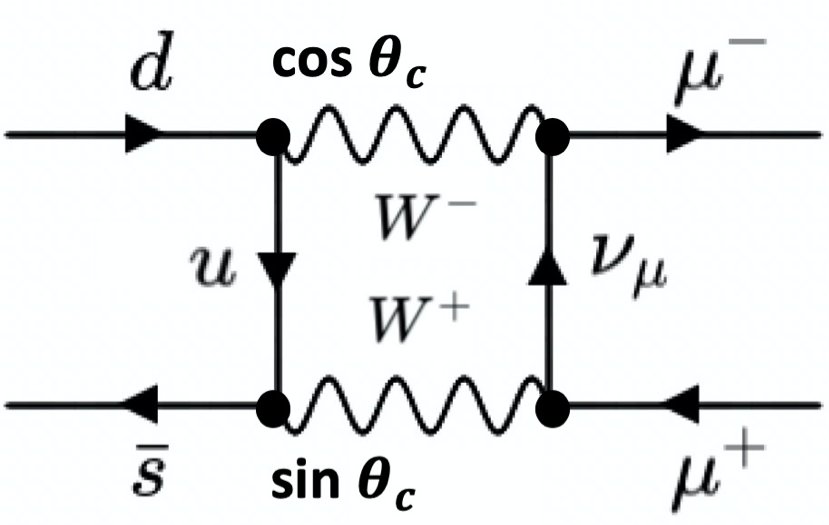
\includegraphics[width=47mm]{Chapters/CH1/figures/kdecay_u}}\qquad
		\subfigure[]{\label{fig:Kdecay_c}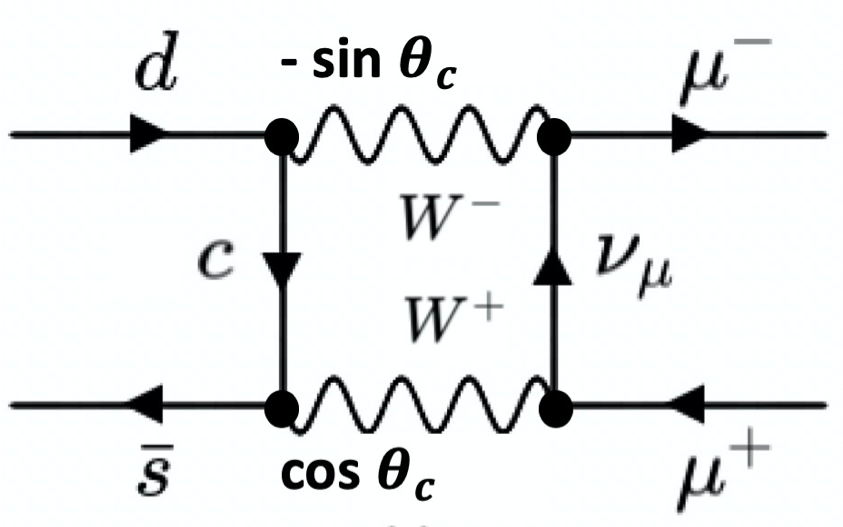
\includegraphics[width=47mm]{Chapters/CH1/figures/kdecay_c}}
	\caption{Feynman diagrams of $K^{0}_{L}\rightarrow \mu^{+} \mu^{-}$ via ($a$) u-quark exchange and ($b$) c-quark exchange}
\end{figure}
In addition to this major prediction, the GIM mechanism led to the prediction that FCNC processes are forbidden at tree-level Leading Order. The branching ratios of several FCNC decays of the top quark in the SM are given in Table~\ref{tab:SM_BR}
\begin{table}[h]
	\begin{adjustbox}{max width=1.\textwidth,center}
		\begin{tabular}{|c|c|c|c|c|c|c|c|c|}
		\hline 
  & $ t\rightarrow uZ$    & $ t\rightarrow cZ$    & $ t\rightarrow u\gamma$ & $ t\rightarrow c\gamma$ & $ t\rightarrow ug$       & $ t\rightarrow cg$       & $ t\rightarrow uH$     & $ t\rightarrow cH$  \\ 
	\hline 
	BR & $8\times 10^{-17} $ & $1\times 10^{-14} $ & $3.7\times 10^{-16} $       & $4.6\times 10^{-14} $      & $3.7\times 10^{-14} $  & $4.6\times 10^{-12} $ & $2\times 10^{-17} $  &$3\times 10^{-15} $  \\ 
		\hline 
		\end{tabular} 
	\end{adjustbox}
\caption{Branching ratios for top quark FCNC interactions in the SM~\cite{aguilar}.}
\label{tab:SM_BR}
\end{table}
\noindent The FCNC production is sensitive to numerous new physics models, as is mentioned in more details in Section \ref{sec:bsm}.\\
The GIM hypothesis represents a generalization of Cabibbo's idea. The introduction of the fourth quark (c) restored the symmetry
in the (then known)  numbers of quark and leptons.\\
These ideas were extended by Kobayashi and Maskawa (1973), who introduced a framework of six quarks and it will be described in the next section.

\subsubsection{CKM matrix}
\label{sec:ckm}
In 1973 Kobayashi and Maskawa extended the Cabibbo's mechanism allowing to describe the transitions within and in-between 3 generations of quarks
using the so-called \textit{CKM} $3\times3$ matrix~\cite{cabibbo,ckm}, which relates the weak eigenstate of down-type quarks to their mass eigenstate:
\begin{equation}
	\begin{pmatrix}
	d' \\ 
	s' \\ 
	b' 
	\end{pmatrix} 
	= V_{CKM}
	\begin{pmatrix}
	d \\ 
	s \\ 
	b
	\end{pmatrix} 
	=
	\begin{pmatrix}
	|V_{ud}| & |V_{us}| & |V_{ub}| \\ 
	|V_{cd}| & |V_{cs}| & |V_{cb}| \\ 
	|V_{td}| & |V_{ts}|  &| V_{tb}|
	\end{pmatrix} 
	\begin{pmatrix}
	d \\ 
	s \\ 
	b
	\end{pmatrix} 
\end{equation}
By  convention, the up-type quarks are taken to be pure states.
Therefore, partners of the up-type quarks within the weak isospin doublets are the weak eigenstates d’, s’ and b’ which are the pure states. \\
The CKM matrix is fully defined by 4 independent parameters, which must be determined experimentally. These parameters are: 3 mixing angles and 1 CP-mixing
phase, which violates the CP\footnotemark symmetry in the SM~\cite{cp_vio}.
The diagonal elements of the CKM matrix are close to 1, reflecting the fact that transitions are favoured between quarks of the same generation. 
The CKM matrix is unitary, i.e. the sum of the transition probabilities for any quark flavour is equal to 1. If this assumption was to be disproved, 
it could imply the existence of a fourth quark generation.
\footnotetext{Charge transformation followed by a parity transformation.}

%\vspace{1cm}
%\textbf{METTERE Electroweak symmetry breaking ???}
%\clearpage
%\subsection{Electroweak symmetry breaking}  METTERE ???

\section{Top quark physics}
The heaviest known elementary particle described by the Standard Model is the top quark.\\
In 1995, the top quark discovery at FERMILAB~\cite{CDF,D0} was a great success for the SM predictions e.g. the corroboration of existence  of a weak isospin partner of the top quark.
Due to its large mass, the predicted lifetime $\mathrm{\tau_{t} \approx 5\times 10^{−25}}$ s (in agreement with theoretical expectations~\cite{LHcb_top}) entails that it decays before hadronising.\\
In the next sections, the production mechanism is reported, as well as an overview of the decay channels.
\subsection{Production}
The top quark can either be produced as pairs, via strong interaction, or as a single top quark via electroweak interaction that does not preserve the flavour.\\
The main parton sub-processes that lead to top-pair production are the quark-antiquark annihilation ($q\bar{q}\rightarrow t\bar{t}$, Figure~\ref{fig:top_prod_a}) and the gluon-gluon fusion ($gg\rightarrow t\bar{t}$, \Cref{fig:top_prod_b,fig:top_prod_c}).\\
\begin{figure}[h]
	\centering
	\subfigure[]{\label{fig:top_prod_a}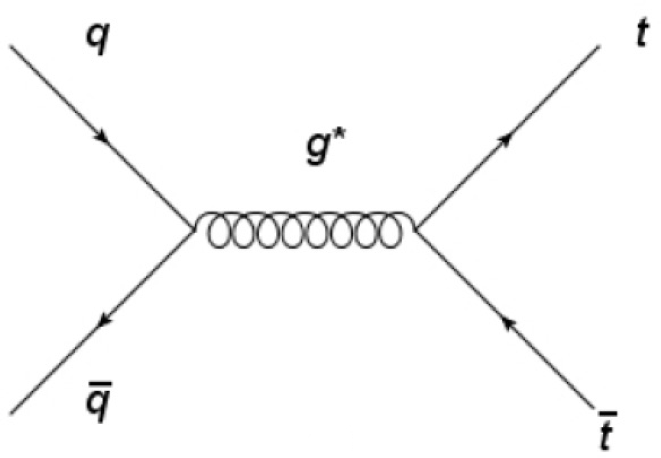
\includegraphics[width=37mm]{Chapters/CH1/figures/top_prod_a}}\quad
	\subfigure[]{\label{fig:top_prod_b}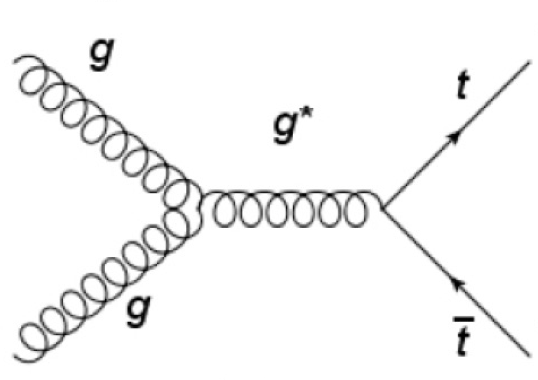
\includegraphics[width=35mm]{Chapters/CH1/figures/top_prod_b}}\quad
	\subfigure[]{\label{fig:top_prod_c}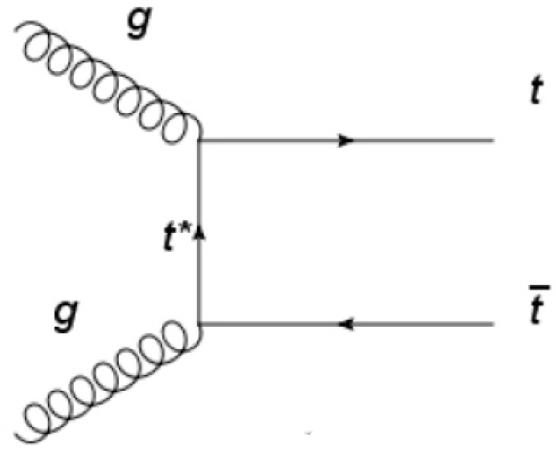
\includegraphics[width=33mm]{Chapters/CH1/figures/top_prod_c}}
	\caption{Feynman diagrams of $t\bar{t}$ production via \subref{fig:top_prod_a} quark-antiquark annihilation ($q\bar{q}\rightarrow t\bar{t}$), \subref{fig:top_prod_b} and \subref{fig:top_prod_c} gluon-gluon fusion ($gg\rightarrow t\bar{t}$) }
\end{figure}
\newline Since in protons there are no valence antiquark, the quark-antiquark annihilation is suppressed by 
the parton distribution functions (PDF) of the antiquark in the proton. Therefore, at the LHC the dominant process turns out to be the
gluon-gluon fusion, while in a proton-antiproton collider, such as Tevatron,
the dominant process is the quark-antiquark annihilation, in fact, at $\sqrt{s}= 7\,\TeV$:
\begin{itemize}
	\item Tevatron: $q\bar{q}\rightarrow t\bar{t} \approx 85\%$, $gg\rightarrow t\bar{t} \approx 15\%$
	\item LHC: $q\bar{q}\rightarrow t\bar{t} \approx 20\%$, $gg\rightarrow t\bar{t} \approx 80\%$
\end{itemize}
Top-pairs can be produced also by the weak interaction when two quarks exchange $Z^0$ or a $\gamma$; however the cross-section of these
type of processes is negligible when compared to the production cross-section through strong interaction.\\
Although at the LHC the top quarks are mainly produced in the process described above, a non negligible number of tops 
are produced singly by weak interaction. The production cross section, in this case, is equal to approximately 1/3 of the top-pair production
cross-section, which is $\sigma_{t\bar{t}} = 831.8^{+19.8+35.1}_{-29.2-35.1}$ pb~\cite{pdg}, at $\sqrt{s}=13$ TeV and for a top quark mass of 172.5 \GeV.

\subsection{Decay channels}
Since the top quark mass is larger than the W boson mass, the top decays through the weak interaction, mainly in to $t\rightarrow W^{+}b$; according to the SM in 100\% of the possible cases.\\
The other channels ($t\rightarrow W^{+}s$, $t\rightarrow W^{+}d$) are strongly suppressed by the CKM matrix elements (see Section \ref{sec:ckm}). Exploiting the matrix unitarity 
and the B meson oscillation measurements, it is possible to extract the following BRs\cite{tdecayBR}:
\begin{table}[!ht]
	\centering
	\begin{tabular}{l}
		%\hline
		BR$(\mathrm{t \rightarrow W^{+} b)\sim 0.998}$\\
		%\hline
		BR$(\mathrm{t \rightarrow W^{+} s)\sim 1.9\cdot10^{-3}}$\\
		%\hline
		BR$(\mathrm{t \rightarrow W^{+} d)\sim 10^{-4}}$\\
		%\hline
	\end{tabular}
\end{table}
\newline Therefore, the top decay total width is given by, in good approximation, the decay $(t \rightarrow W^{+} b)$, thus it equals to $\Gamma_t = 1.44$~GeV.
The W boson may decay in only two ways: "leptonically" \\($W\rightarrow l\nu$) or "hadronically" ($W\rightarrow q\bar{q}'$). This leads to three different categories
of $t\bar{t}$ decays: dileptonic, semi-leptonic or hadronic.\\ Figure~\ref{fig:ttBR} summarizes the BRs associated to each channel.\\
At hadron colliders, the dominant hadronic mode is the most difficult to isolate due to the large QCD background.
\begin{figure}[!h]
	\centering
	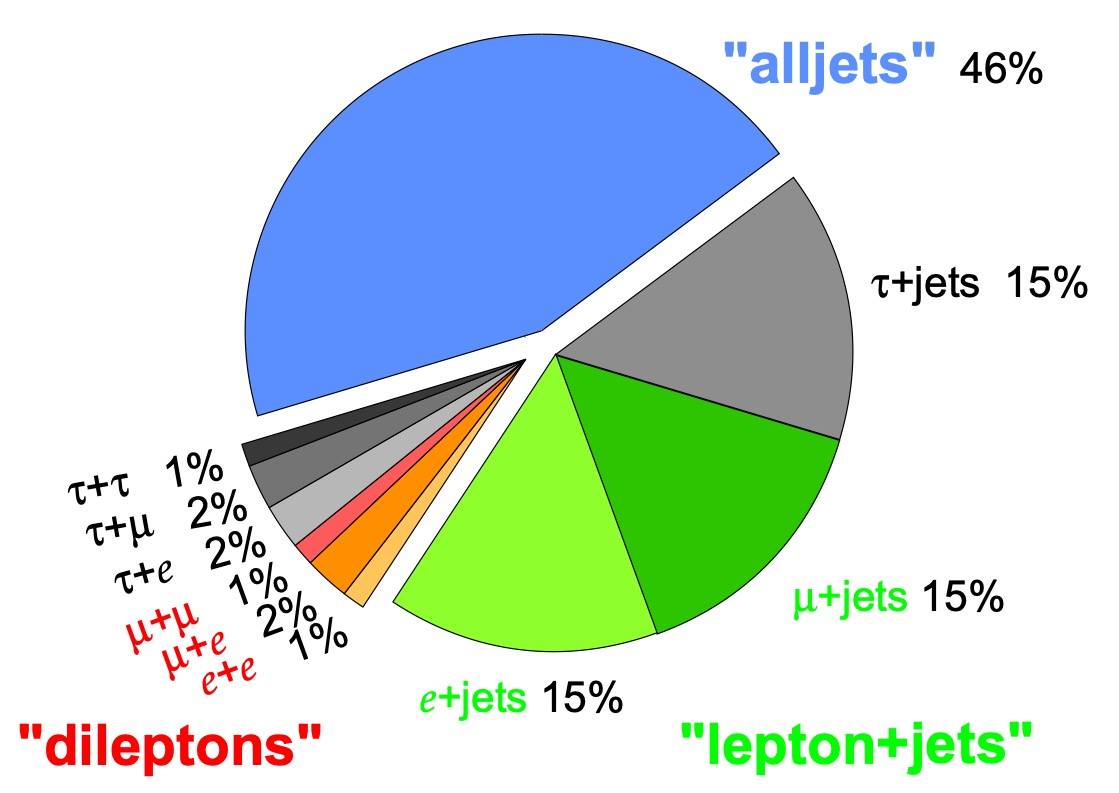
\includegraphics[width=0.55\textwidth]{Chapters/CH1/figures/ttBR}
	\caption{Branching rations associated to each $t\bar{t}$ decay channel \cite{ttdecayBR}.}
	\label{fig:ttBR}
\end{figure}

\newpage
\section{Physics motivation}
The heaviest particle in the Standard Model (SM), the top quark, decays almost exclusively to a \PW-boson and a bottom quark~\cite{pdg2}. %In proton--proton ($pp$) collisions, top quarks are produced dominantly in pairs, via the strong interaction, but also singly, via the electroweak interaction. \\%involving a $Wtb$ vertex. %Therefore single-top quark production provides a powerful probe of the electroweak couplings of the top quark. 
Within the SM, "flavour-changing neutral-current" (FCNC) processes are forbidden at tree level due to the Glashow-Iliopoulos-Maiani mechanism \cite{gim} (see Section~\ref{sec:gim}) and the approximate diagonality of the Cabibbo-Kobayashi-Maskawa matrix~\cite{pdg2} causes the suppression of such processes at higher orders (see Section~\ref{sec:ckm}).\\
Nonetheless, there are several scenarios beyond the Standard Model (BSM) that can significantly enhance the FCNC processes in the top quark sector, opening a door for its detection at the Large Hadron Collider (LHC)~\cite{aguilar,barger,h2dm_limit,mssm_limit,RPV_limit, extra_limit} and some of them will be discussed in Section~\ref{sec:bsm}. \\
The analysis presented in the following details a search for FCNC $\Pqt\rightarrow \PZ\Pqc$ decay. 
%A comparison between SM and BSM predictions for the branching ratios of top quark decays to an up or a charm quark and a \PZ boson is shown in Table \ref{tab:intro-fcnc-br-th}.\\
%
%\begin{table}[h]
%	\begin{adjustbox}{max width=1.\textwidth,center}
%		\begin{tabular}{ccccccccc}
%			\hline 
%			Model:&  			                         SM&  				   QS&  			   2HDM&  				FC 2HDM				& MSSM 			&  RPV SUSY			&  			RS				& EMF \\ 
%			\hline 
%			$\mathcal{B}(t\rightarrow qZ)$ & $10^{-14}$     & $10^{-4}$ &  $10^{-6}$          & $10^{-10}$  & $10^{-7}$      &$10^{-6}$            & $10^{-5}$           & $10^{-6}$  \\ 
%			\hline 
%		\end{tabular} 
%	\end{adjustbox}
%	\caption{Maximum allowed FCNC $t\rightarrow qZ$, ($q$ = $u$, $c$) branching ratios predicted by several models\cite{tcZ_sm,qs_limit,h2dm_limit,mssm_limit,RPV_limit,extra_limit,rs_limit,report_limit}.}
%	\label{tab:intro-fcnc-br-th}
%\end{table} 

\noindent In a model independent way, the anomalous couplings can be described by the so called effective field theory (EFT).
This theory considers an extension of the SM Lagrangian $\mathcal{L}_{SM}$ by operators in higher-dimensions of the mass, suppressed by the scale of new physics $\Lambda$ as shown in \Cref{eq:lagrangian}.
Dimension-5 operators are not considered in this analysis due to the introduction of lepton-flavour violating processes. 
Therefore, the anomalous couplings can be approximated with dimension-6 operators $O_{i}^{(6)}$ whose strength  is given by the Wilson coefficients $C_{i}^{(6)}$.\\

\begin{equation}
\mathcal{L} = \mathcal{L}_{SM} + \frac{1}{\Lambda^2}\sum_{i} C_{i}^{(6)} O_{i}^{(6)}  
\label{eq:lagrangian}
\end{equation}

\noindent Experimental limit on the branching ratio of FCNC $\mathrm{\Pqt\rightarrow\PZ\Pqc}$ decays was previously established by experiments at the Large Electron-Positron Collider (LEP)~\cite{ALEPH,DELPHI,OPAL,L3}, the Hadron-Electron Ring Accelerator (HERA)~\cite{ZEUS}, the Tevatron\ \cite{CDF,DZero} and the Large Hadron Collider (LHC)~\cite{TOPQ-2017-06,Chatrchyan:2013nwa,CMS-TOP-12-039}. The ATLAS and the CMS collaborations obtained limits at the \SI{95}{\percent} confidence level (CL) for this process using data collected at $\sqrt{s}$ = \SI{13}{\TeV} and $\sqrt{s}$ = \SI{8}{\TeV}, focusing on FCNC top-quark decays~\cite{TOPQ-2017-06,Chatrchyan:2013nwa}, or both production and decay modes combined~\cite{CMS-TOP-12-039}. 
A summary of the ATLAS and CMS results on the limits on FCNC couplings is shown in \Cref{fig:intro:limits}. The actual observed limits on the FCNC \tZc coupling from ATLAS is $\mathrm{BR(t\to cZ) < \SI{2.4e-4}{}}$~\cite{TOPQ-2017-06}.\\
Recent studies were done on the interference effects on the FCNC \textit{tZq} and $t\gamma q$ couplings in single-top production and $\mathrm{t\bar{t}}$ decay, concluding that these effects are smaller than the variations of the systematics uncertainties considered~\cite{Interference}. Therefore, both decay and production modes are taken into account in this analysis to improve the results on the limit for \tZc anomalous coupling.

\begin{figure}[htb]
	\centering
	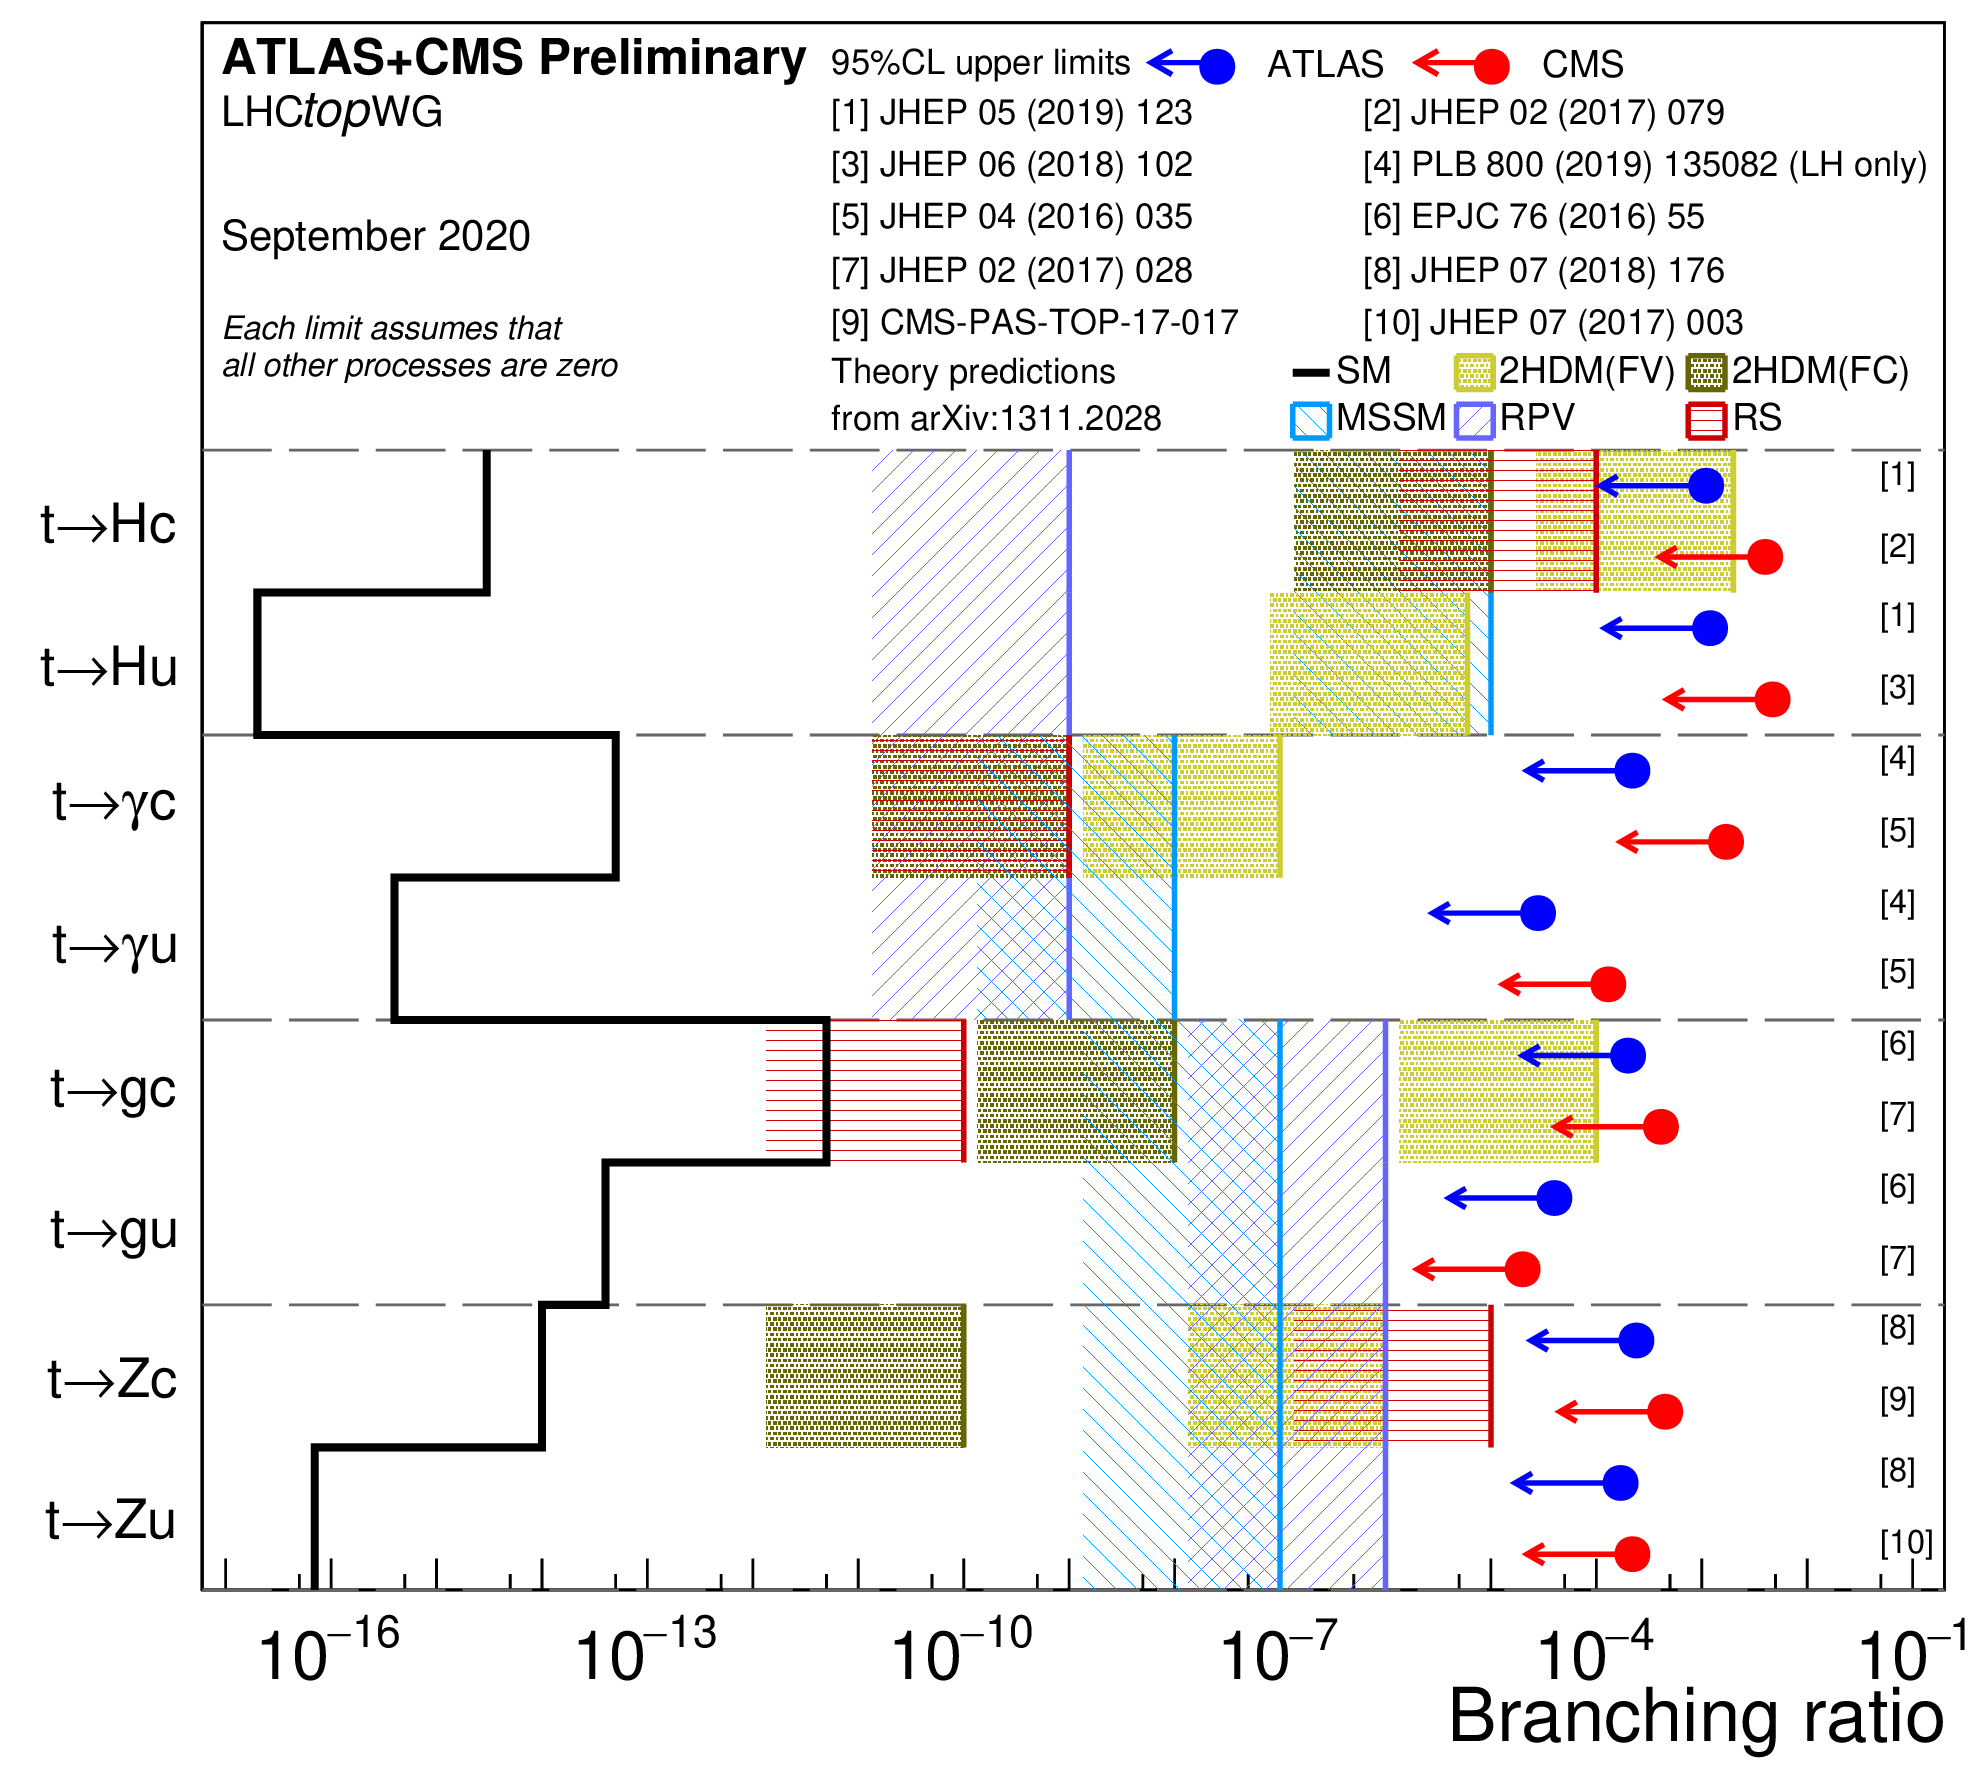
\includegraphics[scale=0.15]{Chapters/CH5/figures/fcnc_summarybsm}
	\caption{Summary of the current 95\% confidence level observed limits on the branching ratios of the top quark decays via flavour changing neutral currents to a quark and a neutral boson $t\rightarrow Xq$ ($X = g, Z, \gamma,$ or $H$; $q = u$ or $c$) by the ATLAS and CMS Collaborations compared to several new physics models. The ATLAS limits on $t \rightarrow q$ are valid for the case of a purely left-handed coupling. Status of figure: September 2020~\cite{lim_2020}.}
	\label{fig:intro:limits}
\end{figure}

\section{Theories for physics beyond the Standard Model}
\label{sec:bsm}
The previous sections described the core components of what we call \textit{Standard Model} and report few major successes of many. 
Its predictive power makes this model the most tested in physics and it reached the culmination of success on 4 July 2012, when
the ATLAS and CMS experiments at CERN announced the observation a new particle in the mass region around 125~GeV, the
Higgs boson~\cite{higgsDiscovery}. \\
But in spite of its important achievements, the SM falls short of explaining several important observations that in this section
are briefly reported.
\begin{itemize}
\item The SM considers neutrinos as massless particles but this is in contradiction with the results of many experiments, which observed,
in several different contexts, the \textit{neutrino oscillations}. 
It is a quantum mechanical phenomenon whereby a neutrino created with a specific lepton family number ($e$, $\mu$, or $\tau$) 
can later be measured to have a different lepton family number and this mechanism, implies that the neutrino has a non-zero mass 
since it arises from mixing between the flavour and mass eigenstates of neutrinos. 
\item The SM can not describe \textit{dark matter} and \textit{dark energy}. The first evidence of dark matter came with the observation of 
the rotational speed of galaxies, which suggests the existence of a huge amount of undetected mass~\cite{zwicky}.\\
None of the SM particles could explain this phenomenon and, since a dark matter has never been directly observed, implies that
it interacts only weakly with the ordinary matter and radiation, or does not interact at all.\\
Likewise, dark energy is an unknown form of energy that affects the universe on the largest scales.
The first observational evidence for its existence came from supernovae measurements, which showed that the universe does 
not expand at a constant rate; rather, the expansion of the universe is accelerating.\\
The data collected by the Planck spacecraft, indicate that dark energy contributes  68\% of the total energy in the present-day observable universe. 
The mass–energy of dark matter and ordinary (baryonic) matter contributes 27\% and 5\%, respectively, and other components 
such as neutrinos and photons contribute a very small amount~\cite{plank}. 
\item After the Big Bang one could expect that the universe produced the same amount of particles-antiparticles and that the constant annihilation
of pairs would have resulted in a universe of radiation. What we observe actually is large cosmological matter (but not antimatter) structures.
The mechanism suggested by the SM through the CP-symmetry violation of neutral oscillating hadrons is not sufficient to explain alone this phenomenon.
\item There are also other strong indications that the SM could be not yet complete. Indeed, it is based on 19 parameters (excluding neutrino masses)
that must be determined experimentally and have no known theoretical origin.  Moreover, gravity could not be included as a gauge theory because, 
describing graviton (the associated gauge boson) interactions, the classical theory of  Feynman diagrams, and semiclassical corrections with 
at least two loops lead to \textit{ultraviolet divergences}. These infinite results cannot be removed 
because quantized general relativity is not perturbatively renormalizable, unlike QED and models such as the Yang–Mills theory. 
Therefore, when the probability of a particle to emit or absorb gravitons is calculated, the theory loses predictive veracity. 
Those problems and the complementary approximation framework are grounds to show that a theory more unified than quantized general relativity is 
required to describe the behaviour near the Planck scale. 
\item The problem of \textit{naturalness} is also much debated in literature. The Higgs boson is very sensitive to loop corrections and if one considers the theory close to the Planck scale, the corrections involving the top quark may not explain why the Higgs boson mass is so relatively small ($\sim$125 GeV). Another problem is, in fact, the mass scale of fermions that ranges across many orders of magnitude without any clear explanation.
\end{itemize}
There are many models of "new physics" that attempt to describe and explain the phenomena mentioned above but so far there is no evidence of new physics Beyond Standard Model (BSM). 
In the SM, top quark decays almost exclusively into $bW$ while flavour-changing neutral current (FCNC) decays such as $t\rightarrow qZ$ are forbidden at tree level. 
FCNC decays occur at one-loop level (Figure~\ref{fig:tqZ_fey}) but are strongly suppressed by the GIM mechanism (Section \ref{sec:gim}), with a suppression factor of 14 orders of
magnitude relative to the dominant decay mode\cite{tcZ_sm}.
\begin{figure}[!h]
	\centering
	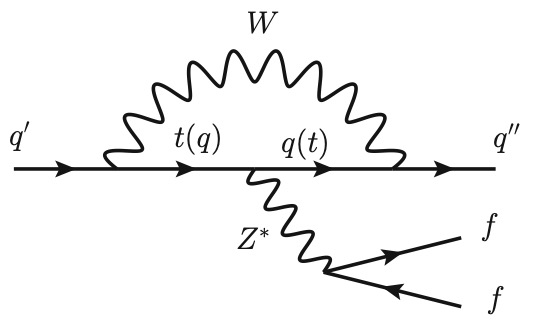
\includegraphics[width=0.5\textwidth]{Chapters/CH1/figures/tqZ_fey}
	\caption{Sketched Feynman diagram for SM $q' \rightarrow q'' f \bar{f}$ induced by the $tqZ$ coupling, where $q'$ and $q''$ denote the down-type quarks; $q = u, c$, and $f$ can be any possible fermions. In the Standard Model, FCNC processes are forbidden at tree level but occur at one-loop level (see GIM mechanism in Section \ref{sec:gim}).}
	\label{fig:tqZ_fey}
\end{figure}

\noindent However, in the BSM models, the suppression could be relaxed and the loop diagrams mediated by new bosons that could contribute, 
leading to couplings of many orders of magnitude higher than those expected by the SM.\\
Examples of such extensions are the quark-singlet model (QS)\cite{qs_limit}, the two-Higgs-doublet model with (FC 2HDM) or without (2HDM) flavour conservation\cite{h2dm_limit},
the Minimal Supersymmetric Standard Model (MSSM)\cite{mssm_limit}, the MSSM with R-parity violation (RPV SUSY)\cite{RPV_limit}, models with warped extra dimensions (RS)\cite{extra_limit}, or extended mirror fermion models (EMF)~\cite{rs_limit}.
Reference~\cite{report_limit} gives a comprehensive review of the various extensions of the SM that have been proposed.
Table~\ref{tab:expBR} provides the maximum values for the branching ratios  predicted by these models and compares them to the value predicted by the SM.\\
In this section we will briefly describe some of these theories interesting for the topics of this thesis.
\begin{table}[!h]
	\begin{adjustbox}{max width=1.\textwidth,center}
		\begin{tabular}{ccccccccc}
			\hline 
			Model:&  			                         SM&  				   QS&  			   2HDM&  				FC 2HDM				& MSSM 			&  RPV SUSY			&  			RS				& EMF \\ 
			\hline 
			$\mathcal{B}(t\rightarrow qZ)$ & $10^{-14}$     & $10^{-4}$ &  $10^{-6}$          & $10^{-10}$  & $10^{-7}$      &$10^{-6}$            & $10^{-5}$           & $10^{-6}$  \\ 
			\hline 
		\end{tabular} 
	\end{adjustbox}
\caption{Maximum allowed FCNC $t\rightarrow qZ$, ($q$ = $u$, $c$) branching ratios predicted by several models\cite{tcZ_sm,qs_limit,h2dm_limit,mssm_limit,RPV_limit,extra_limit,rs_limit,report_limit}.}
\label{tab:expBR}
\end{table} 

\subsection{Quark singlets}
The need to suppress the FCNC processes is motivated by the fact that:
\begin{itemize}
	\item they are not mediated by $Z^0$ boson at tree-level
	\item no FCNC mechanism is in the scalar sector at tree-level 
\end{itemize}
It is possible to overcome these dogmas using extensions of the SM, like the Quark Singlets (QS)~\cite{barger} that introduces a vector-like quark ($\mathrm{Q=\frac{1}{3}}$ or $\mathrm{Q=\frac{2}{3}}$), thus a small violation of the $\mathrm{3 \times 3}$ $V_{CKM}$ unitarity (see Section \ref{sec:ckm}), mediated by $Z^0$ boson and natural 
FCNC suppression at tree-level.
\vspace{\baselineskip}
\\Given $x_L$ and $x_R$, $SU(2)_{L}$ singlets
\begin{equation}
\begin{pmatrix}
d' \\ 
s' \\ 
b' \\
x' 
\end{pmatrix} 
=
\begin{pmatrix}
|V_{ud}| & |V_{us}| & |V_{ub}|  & |V_{ux}| \\ 
|V_{cd}| & |V_{cs}| & |V_{cb}|   & |V_{cx}| \\ 
|V_{td}| & |V_{ts}|  &| V_{tb}|   & |V_{tx}|
\end{pmatrix} 
\begin{pmatrix}
d \\ 
s \\ 
b \\
x
\end{pmatrix} ,
\end{equation}
the non orthogonality of the columns leads to terms of the type:
\begin{equation}
J_{\mu}= \frac{g}{cos\theta_W}Z_{bd}\bar{b}_{L}\gamma_{\mu}d_{L}Z^{\mu}
\end{equation}
where
\begin{equation}
Z_{bd}=V_{ud}V^*_{ub}+V_{cd}V^*_{cb}+V_{td}V^*_{tb}
\end{equation}
and $Z_{bd}$ is suppressed by $\frac{m_q}{m_x}$.
\vspace{\baselineskip}
\\In this way it is possible to have deviations from $\mathrm{3 \times 3}$ unitarity.\\
For instance, the PMNS matrix in the leptonic sector, in the context of the see-saw mechanism is not  $\mathrm{3 \times 3}$ unitarity~\cite{pnms}.
\\Vector-like quarks provide the simplest model with spontaneous \textit{CP violation} and a framework to have a common origin
of all CP violation, because it is a potential solution of the \textit{strong CP problem}.

\subsection{Two Higgs Doublet Model}
The LHC discovery of a Standard-Model-like Higgs H(125) particle in 2012\cite{higgsDiscovery} could be a portal to an extended Higgs sector predicted by several models. One of such models is the Two-Higgs-Doublet Model (2HDM)~\cite{h2dm}.
The most natural extension of the Standard Model scalar sector is the addition of an
extra $SU(2)_{L}$ doublet. 
\vspace{\baselineskip}
\\The 2HDM is an \textit{Effective Field Theory} (EFT\footnotemark) 
\footnotetext{ An EFT corresponds to a low-energy approximation to
a more fundamental underlying theory, characterized by an energy scale $\Lambda$ (e.g. the mass
of new particles)}
consisting of two complex Higgs doublets, which provide masses to both the up-type and the down-type fermions:
\begin{equation} 
	\Phi_{1}= \binom{\phi^{+}_{1}}{\phi^{0}_{1}}  \qquad \Phi_{2}= \binom{\phi^{+}_{2}}{\phi^{0}_{2}}
\end{equation}
with the minimum of the potential corresponding to
\begin{equation} 
	\Phi_{1,0}= \frac{1}{\sqrt{2}}\binom{0}{\nu_1}  \qquad \Phi_{2,0}= \frac{1}{\sqrt{2}}\binom{0}{\nu_2}.
\end{equation}
\\After the electroweak symmetry breaking (EWSB),
there are five physical scalar fields, consisting of neutral bosons $h,H,A$ of which the
first two bosons are CP-even, as opposed to the A-boson which is CP-odd and of two charged Higgs states $H^{\pm}$.
\\The model is parametrized by the five Higgs masses ($m_H$, $m_h$, $m_{H^{\pm}}$, $m_A$), the ratio of the vacuum expectation 
values of the two Higgs doublets $\tan{\beta}= \nu_{2}/\nu_{1}$ and the mixing angle $\alpha$ between the CP-even Higgs states.
\\There exist four types of 2HDM which simultaneously forbid the presence of FCNC and preserve CP symmetry:
\begin{itemize}
	\item in Type I all fermions couple to the second doublet $\Phi_2$. It follows that BR are independent of $\tan{\beta}$;
	\item in Type II or MSSM-like scenario, lepton and down-type quarks couple to the first doublet $\Phi_1$, whilst up-type quarks couple to $\Phi_2$;
	\item in Type III or lepton specific scenario, quarks couple to  $\Phi_2$ while leptons couple to the other doublet;
	\item in Type IV or flipped model, the coupling of the leptons is reversed with respect to the Type-II model.
\end{itemize}	
	
\subsection{Minimal Supersymmetric Standard Model}
The FCNC processes have also been studied within the \textit{Minimal Supersymmetric Standard Model} (MSSM), where there are loop corrections of the supersymmetric QCD with gluinos 
and scalar quarks, as shown in Figure~\ref{fig:fey_mssm}.
\begin{figure}[!h]
	\centering
	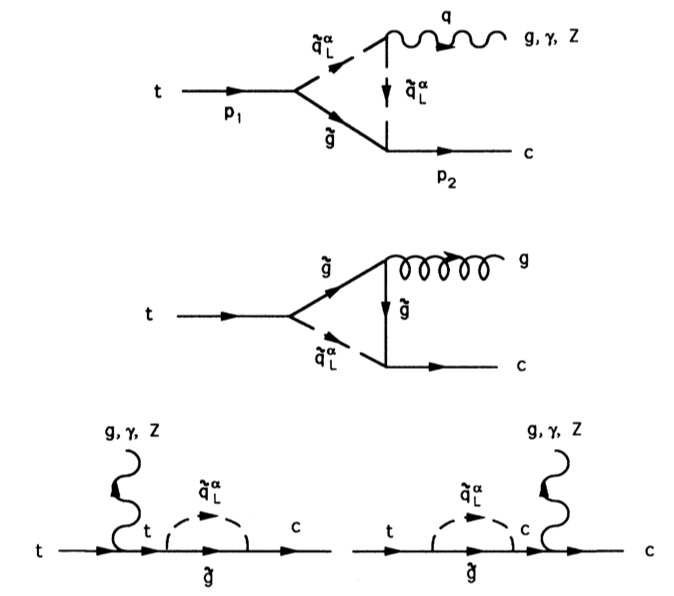
\includegraphics[width=0.55\textwidth]{Chapters/CH1/figures/fey_mssm}
	\caption{The diagrams with scalar quarks and gluinos within the loop, which contribute to the top quark decay into a charm quark and a Z boson, photon, or gluon\cite{coulture_mssm}.}
	\label{fig:fey_mssm}
\end{figure}
In supersymmetric QCD it was shown that there occurs flavour-changing strong interactions between the gluino, the left-handed quarks, and their supersymmetric scalar
partners, whereas the couplings of the gluino to the right-handed quarks and their partners remains flavour diagonal.
To calculate the one-loop diagrams shown in Figure~\ref{fig:fey_mssm}, we need the couplings of the gluon to the gluinos, of the
scalar partners of the left-handed quarks to the gluon, photon, and Z boson, and of the gluino to the left-handed quark and its scalar partner.\\
After the introduction of non-trivial squark mixing, it is possible to calculate the coupling that leads to flavour changing in which appears $K_{ij}$, the supersymmetric version of $V_{CKM}$:
\begin{equation}
\begin{pmatrix}
	1                  & \epsilon   & \epsilon^2 \\ 
	-\epsilon     & 1              & \epsilon \\ 
	-\epsilon^2 & -\epsilon & 1
\end{pmatrix} .
\end{equation}
It is possible to demonstrate that all divergent terms cancel exactly, without the GIM mechanism.\\
Finally, we define $\mathcal{B}(t \rightarrow cZ)=\frac{\Gamma_{S}(t \rightarrow cZ)}{\Gamma_{W}(t \rightarrow bW)}$, where:
\begin{equation} 
\Gamma_{W}(t \rightarrow bW) = \frac{\alpha}{16\sin{\Theta_W}} m_{top} \left(1-\frac{m^{2}_{W}}{m^{2}_{top}}\right)^2 \left(2+\frac{m^{2}_{top}}{m^{2}_{W}}\right)
\end{equation}
Using the following values for the parameters $m_{top}=174$~GeV, $\alpha_{s}=1.4675/\ln{\left( \frac{m^{2}_{top}}{\Lambda^{2}_{QCD}} \right)}$ with $\Lambda_{QCD}=0.18$~GeV, it is
possible to derive the branching ratio $\mathcal{B}(t \rightarrow cZ)$ as a function of the scalar mass $m_{S}$ for a gluino mass of 100~GeV (Figure~\ref{fig:BR_mssm}).
\begin{figure}[!h]
	\centering
	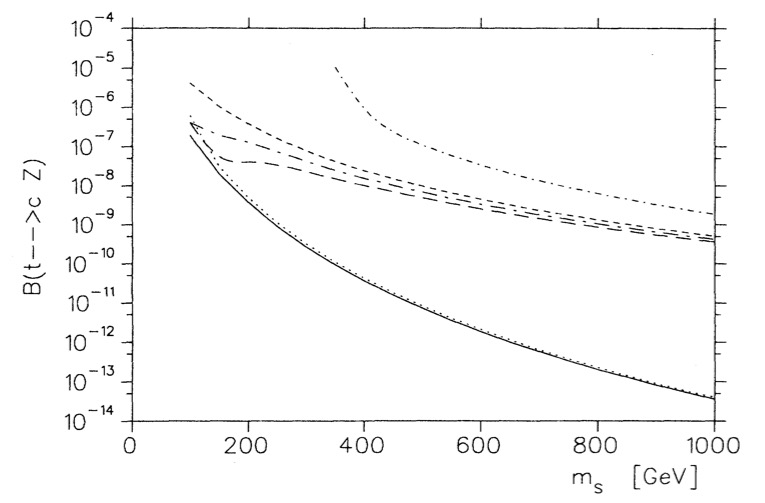
\includegraphics[width=0.65\textwidth]{Chapters/CH1/figures/BR_mssm}
	\caption{The branching ratio $\mathcal{B}(t \rightarrow cZ)$ as a function of the scalar mass $m_{S}$. The gluino mass was taken to be 100~GeV. The solid line is the unphysical case 
		with no squark mixing, the dotted lines are different scenarios of squark mixing\cite{coulture_mssm}.}
	\label{fig:BR_mssm}
\end{figure}
\\We see that without mixing, $\mathcal{B}(t \rightarrow cZ)$ decreases rapidly with increasing scalar mass. The mixing has a drastic effect. It enhances the branching ratio by up to 
5 orders of magnitude for large $m_{S}$.
\clearpage
\let\cleardoublepage\clearpage

